\section[ML overview]{Machine learning overview}

\subsection{}

\begin{frame}
    \frametitle{What is machine learning?}

    \begin{block}{My definition}
        The study of computational algorithms
        \begin{itemize}
            \item that \alert{predict} outputs from inputs;
            \item whose behavior is determined by \alert{model parameters};
            \item that \alert{learn} how to make predictions by fitting (``training'') the model parameters to data;
            \item that \alert{iteratively} improve their model parameters via continual training.
        \end{itemize}
    \end{block}

    \begin{columns}
        \begin{column}{2.5in}
            Simplest example: linear regression
            \begin{itemize}
                \item Sort of: not iterative
                \item Predicts $y$ from $x$ via $y = ax + b$
                \item Two parameters: $a$, $b$
                \item Fitted to data
            \end{itemize}
        \end{column}
        \begin{column}{1.75in}
            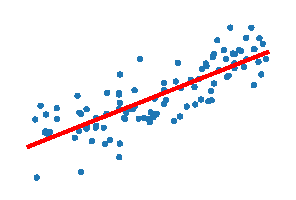
\includegraphics{linear_regression}
        \end{column}
    \end{columns}
\end{frame}

\begin{frame}
    \frametitle{A (much) more complicated example}
    \begin{columns}
        \begin{column}{0.37\textwidth}
            \begin{block}{Image classification}
                A canonical problem: given an image, predict the correct label
            \end{block}
        \end{column}
        \begin{column}{0.63\textwidth}
            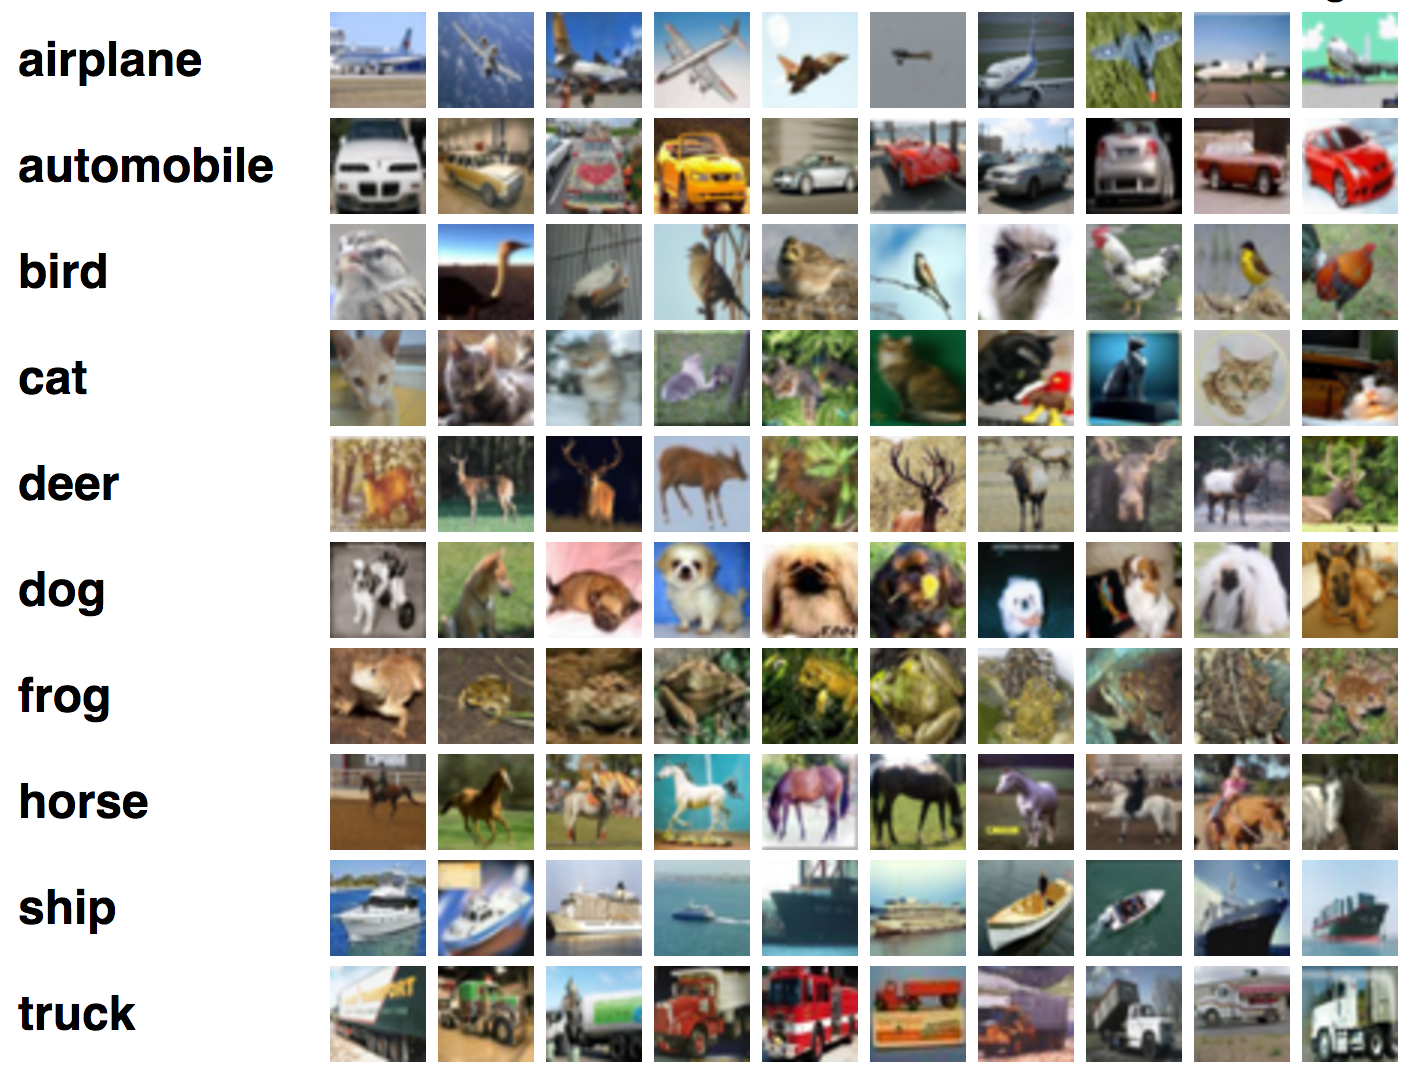
\includegraphics[width=\textwidth]{cifar10}
        \end{column}
    \end{columns}

    \begin{itemize}
        \item Roughly: if a human can do it, a computer should be able to too
        \item More rigorously: $\exists$ a mapping from image pixels to labels
        \begin{itemize}
            \item Mapping too difficult for humans to understand
            \item Let an algorithm model it
        \end{itemize}
    \end{itemize}
\end{frame}

\begin{frame}
    \frametitle{An image classification solution}

    \begin{columns}
        \begin{column}{0.7\textwidth}
            ResNet-152: a 152-layer convolutional neural network with 11.3 billion multiply/adds! \citep{He15}
            \begin{itemize}
                \item Trained on ImageNet data: 14,197,122 images
                \item Iterative training
                \begin{itemize}
                    \item 600,000 training iterations
                    \item At each iteration, model parameters updated based on \emph{mini-batch} of 256 images
                \end{itemize}
                \item Won multiple image classification competitions
            \end{itemize}
        \end{column}
        \begin{column}{0.3\textwidth}
            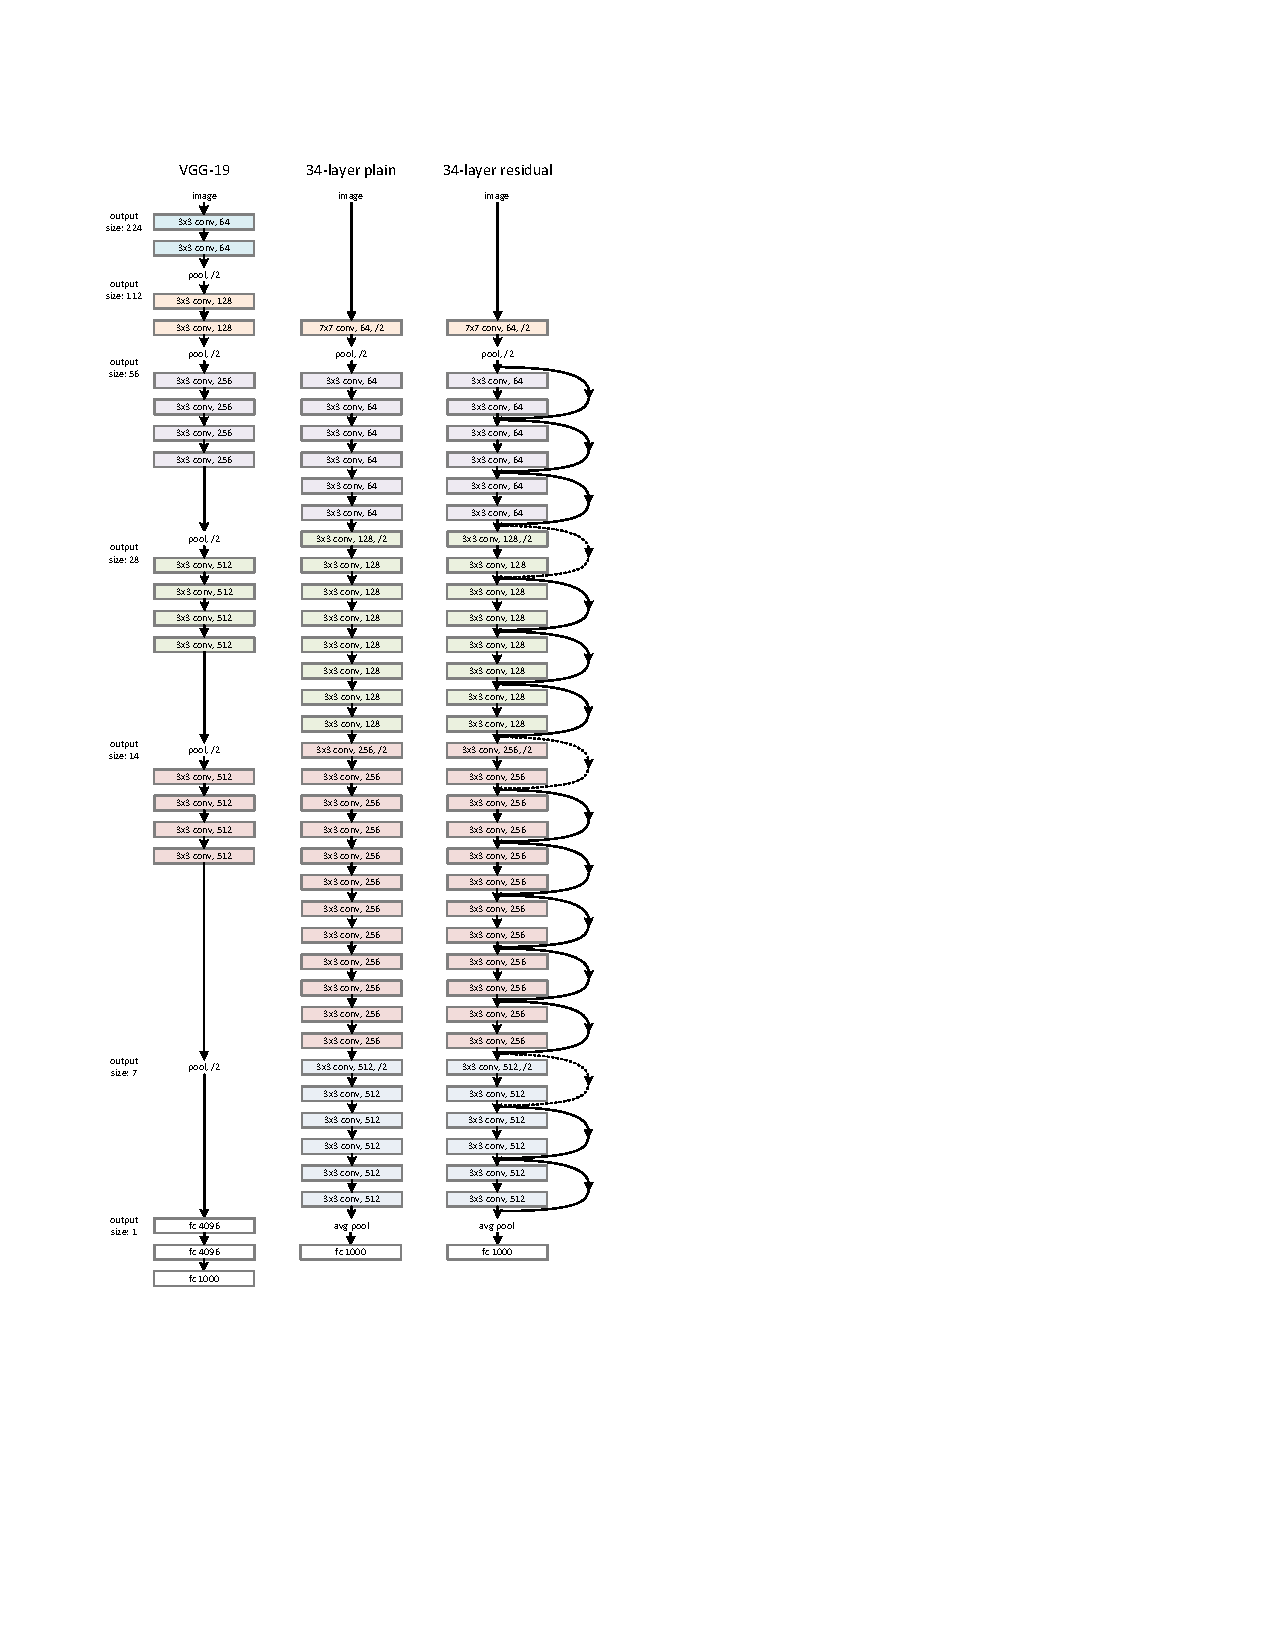
\includegraphics[width=\textwidth]{resnet}
        \end{column}
    \end{columns}
\end{frame}

\begin{frame}
    \frametitle{Supervised learning}

    Machine learning problems/algorithms categorized as \alert{supervised} vs.~\alert{unsupervised}

    \begin{block}{Supervised learning}
        \begin{itemize}
            \item Data represented as $\{(x_i, y_i)\}_{i=1}^n$, with $x_i$ an input and $y_i$ an output
            \item Given $x_i$, predict $y_i$
        \end{itemize}
    \end{block}

    Supervised learning further split into: \\[1ex]
    \begin{columns}[t]
        \begin{column}{0.47\textwidth}
            \alert{Regression}: $y_i$ continuous, e.g.:
            \begin{itemize}
                \item $x_i =$ (age, sex, race, weight, height, LDL, HDL, zip code, etc.), $y_i =$ life expectancy
                \item $x_i =$ (stock price history, market conditions, interest rates, etc.), $y_i =$ tomorrow's stock price
            \end{itemize}
        \end{column}
        \begin{column}{0.45\textwidth}
            \alert{Classification}: $y_i$ discrete, e.g.:
            \begin{itemize}
                \item $x_i =$ lots of pixels; $y_i =$ image label (cat, dog, etc.)
                \item $x_i =$ audio speech sample; $y_i =$ words spoken
                \item $x_i =$ list of movies you like; $y_i =$ whether you like \emph{Interstellar}
            \end{itemize}
        \end{column}
    \end{columns}
\end{frame}

\begin{frame}
    \frametitle{Unsupervised learning}
    \begin{block}{Unsupervised learning}<+->
        \begin{itemize}
            \item Data represented as $\{x_i\}_{i=1}^n$ only: no outputs
            \item \alert{Density estimation}: learn the data's probability distribution
        \end{itemize}
    \end{block}

    \uncover<+->{Related problem: \alert{clustering}---find which clusters data belong to} \\[1ex]

    \uncover<+->{Examples:}
    \begin{itemize}[<.->]
        \item Generative modeling: given pictures of volcanoes, generate new ones that look realistic
        \item Determine if loan/insurance applicant is low/medium/high-risk
    \end{itemize}

    % To do: put in volcano images.
    \only<2>{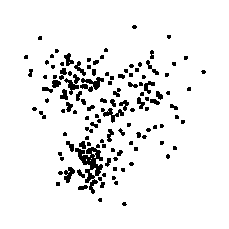
\includegraphics[scale=0.7]{cluster}}
    \only<3->{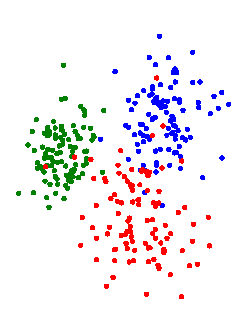
\includegraphics[scale=0.7]{clusters}}
\end{frame}

\begin{frame}
    \frametitle{Notes on supervised vs.~unsupervised learning}

    \begin{itemize}
        \item I will only focus on supervised learning today \& Thursday
        \begin{itemize}
            \item Theory more mature
            \item Techniques more powerful
        \end{itemize}
        \item Many experts believe a strong future in ML requires a shift toward unsupervised learning
        \begin{itemize}
            \item $\exists$ tons of data in the world, but often unlabeled
        \end{itemize}
        \item Semi-supervised learning: usually, small amount of labeled data + lots of unlabeled data
    \end{itemize}
\end{frame}

\begin{frame}
    \frametitle{Machine learning algorithms}

    \begin{columns}
        \begin{column}{0.44\textwidth}
            \uncover<+->{The list is long:}
            \begin{itemize}[<.->]
                \item Logistic regression
                \item Gaussian mixture models
                \item Kernel methods
                \item Naive Bayes classifier
                \item $k$-nearest neighbors, $k$-means, $k$-medians
                \item Decision trees
                \item Random forests
                \item Support vector machines
                \item \alert<+->{(Artificial) neural networks}
                \item Etc.
            \end{itemize}
        \end{column}

        \begin{column}{0.56\textwidth}
            \uncover<.->{%
                I will only focus on neural networks today.
                Even then, variations are plentiful:
            }
            \begin{itemize}[<.->]
                \item \alert<3->{Dense (fully-connected) NN: generic}
                \item Convolutional NN: for spatial data
                \item \alert<3->{Recurrent NN: for temporal data (Thursday's topic)}
                \item Autoencoders: for data representations
                \item Reinforcement learning: for AI/games
                \item Generative models: for making new data
                \item Etc.
            \end{itemize}
            \uncover<.->{These can generally be combined freely}
        \end{column}
    \end{columns}
\end{frame}

%%% Local Variables:
%%% mode: latex
%%% TeX-master: "../nn"
%%% End:
